\chapter{Weighted Temporal Event Graphs: Preserving Causal Paths}
\label{chap:saramaki}

% =============================================================================
\section{Why Static Graphs Fail: A Four-Person Story}
\label{sec:saramaki_motivation}
% =============================================================================

In Chapter~\ref{chap:temporal_networks} we established that a static graph is a
photograph: it records who met whom, but destroys the order in which those
meetings happened. Here we make this failure mode concrete with a small but
illuminating example that we will carry through the entire chapter.

\subsection{Setting the Scene}

Consider four people: \textbf{Alice (A)}, \textbf{Bob (B)}, \textbf{Carol (C)},
and \textbf{Dave (D)}. They have the following four contacts over the course of
four time steps:

\begin{center}
\begin{tabular}{cccl}
\toprule
\textbf{Event ID} & \textbf{People} & \textbf{Time} & \textbf{What happened} \\
\midrule
$e_1$ & Alice -- Bob   & $t = 1$ & Alice and Bob shake hands \\
$e_2$ & Bob -- Carol   & $t = 2$ & Bob and Carol have lunch \\
$e_3$ & Carol -- Dave  & $t = 3$ & Carol and Dave meet at a conference \\
$e_4$ & Alice -- Dave  & $t = 4$ & Alice and Dave attend the same lecture \\
\bottomrule
\end{tabular}
\end{center}

Suppose Alice is \textbf{Patient Zero}. She is infected at $t=0$. What is the
only chain by which she can spread the disease?

\begin{examplebox}{Tracing the Only Valid Transmission Chain}
\begin{itemize}[noitemsep]
    \item Alice is infectious at $t=0$.
    \item At $t=1$, Alice meets Bob. She infects Bob. ($A \to B$)
    \item At $t=2$, Bob meets Carol. He infects Carol. ($B \to C$)
    \item At $t=3$, Carol meets Dave. She infects Dave. ($C \to D$)
\end{itemize}
This is the \textbf{unique valid transmission chain} starting from Alice:
$A \to B \to C \to D$.

What about the contact $e_4$: Alice meets Dave at $t=4$? Dave is
\emph{already infected} from $e_3$, so this meeting does not change the
outcome. However, if Dave had somehow \emph{not} been reached by $e_3$, Alice
\emph{could} infect him directly at $t=4$. Importantly, Alice meeting Dave at
$t=4$ \textbf{could never have caused} the chain $A \to D \to C \to B$,
because Carol already met Dave at $t=3$ --- \emph{before} Alice meets Dave at
$t=4$.
\end{examplebox}

\subsection{What a Static Graph Sees}

Now suppose we forget the timestamps and project the four events onto a static
undirected graph. We keep only the topology: who has ever met whom.

\begin{figure}[H]
\centering
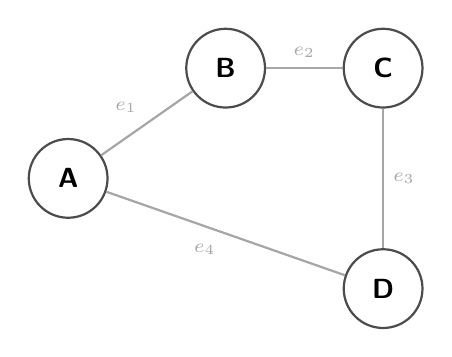
\begin{tikzpicture}[
    pnode/.style={circle, draw=black!70, fill=white, thick,
                  minimum size=1.0cm, font=\bfseries\sffamily},
    sedge/.style={thick, gray!70}
]
    \node[pnode] (A) at (0,0)   {A};
    \node[pnode] (B) at (2,1.4) {B};
    \node[pnode] (C) at (4,1.4) {C};
    \node[pnode] (D) at (4,-1.4){D};

    \draw[sedge] (A) -- node[above left,  font=\scriptsize]{$e_1$} (B);
    \draw[sedge] (B) -- node[above,       font=\scriptsize]{$e_2$} (C);
    \draw[sedge] (C) -- node[right,       font=\scriptsize]{$e_3$} (D);
    \draw[sedge] (A) -- node[below left,  font=\scriptsize]{$e_4$} (D);
\end{tikzpicture}
\caption{The \textbf{static projection} of the four contacts. All edges exist
simultaneously. A graph algorithm sees $A$--$B$--$C$--$D$ and also
$A$--$D$--$C$--$B$, $A$--$D$--$C$--$B$, and so on.}
\label{fig:static_projection}
\end{figure}

On this static graph, every simple path between every pair of nodes is
available. A naive GNN that operates on this graph would conclude, for example,
that the path $D \to C \to B \to A$ is a valid transmission route (Dave infects
Carol, Carol infects Bob, Bob infects Alice). But this is \textbf{physically
impossible}:

\begin{itemize}
    \item Dave only met Carol at $t=3$.
    \item Carol had already met Bob at $t=2$ --- \emph{one time step earlier}.
    \item A pathogen cannot travel backwards in time: Dave cannot have infected
          Carol at $t=3$ and then Carol retroactively infects Bob at $t=2$.
\end{itemize}

\begin{keyinsight}{Static Graphs Create Phantom Paths}
The static projection introduces \textbf{phantom paths} --- paths that look
valid topologically but are causally impossible because the timestamps are
in the wrong order. Any GNN that ignores event timing will learn from these
phantom paths and will be systematically mis-calibrated about the true source.
The core challenge of this entire chapter, and of the Saram\"{a}ki paper, is
to build a data structure that makes it \emph{structurally impossible} to
traverse a phantom path.
\end{keyinsight}

% =============================================================================
\section{The Saram\"{a}ki Insight: Make Events the Nodes}
\label{sec:saramaki_insight}
% =============================================================================

The elegant solution proposed by Saram\"{a}ki, Kivel\"{a}, and Karsai in their
2019 paper ``Weighted temporal event graphs'' \cite{saramaki2019temporal} is a
\textbf{perspective shift} so simple it is almost surprising that it works so
well.

\begin{keyinsight}{The Central Idea: Elevate Events to Nodes}
Instead of treating \emph{people} as graph nodes and \emph{contacts} as edges,
we \textbf{swap the roles}:
\begin{itemize}[noitemsep]
    \item \textbf{People} disappear as primary nodes.
    \item \textbf{Contact events} $(u, v, t)$ become the new nodes of a graph.
    \item \textbf{Causal relationships between events} become directed edges.
\end{itemize}
The result is a new graph --- the \textbf{Temporal Event Graph (TEG)} --- where
the very structure of the graph encodes temporal causality. You cannot traverse
a phantom path because phantom edges simply do not exist in the TEG.
\end{keyinsight}

\subsection{Why This Solves the Problem}

On the original temporal network, phantom paths arise because a GNN cannot
distinguish the \emph{order} of edges incident on a node. Person $B$ is
connected to both $A$ and $C$ in the static graph, and nothing in the adjacency
matrix tells you that $B$ met $A$ first.

In the Temporal Event Graph, the two events ``$B$ meets $A$'' and ``$B$ meets
$C$'' are \emph{separate nodes}. A directed edge from event $e_1=(A,B,t{=}1)$
to event $e_2=(B,C,t{=}2)$ means ``$e_1$ can causally enable $e_2$'' --- which
is precisely true: $B$ was infected at $t=1$ and can pass the virus on at
$t=2$. The reverse edge $e_2 \to e_1$ does not exist, making the phantom path
structurally absent.

\begin{analogybox}{The Train Timetable vs. the Railway Map}
A standard railway map shows you which cities are connected by rail. You might
conclude that you can travel from London to Edinburgh in any order. The
\emph{timetable}, however, makes an explicit graph of which trains you can
catch after getting off another train. If Train A arrives at Birmingham at
12:00 and Train B departs Birmingham at 11:30, there is no edge from Train A
to Train B in the timetable graph --- the connection is physically impossible.
The Temporal Event Graph is the timetable. The static projection is the map.
\end{analogybox}

\subsection{Our Four Events as Nodes}

Let us apply this idea to the Alice/Bob/Carol/Dave example. We have four
events. In the TEG, these become four nodes:

\begin{center}
\begin{tabular}{ccccc}
\toprule
\textbf{TEG Node} & \textbf{Original Event} & \textbf{People} & \textbf{Time} \\
\midrule
$v_{e_1}$ & $e_1$ & Alice, Bob   & $t=1$ \\
$v_{e_2}$ & $e_2$ & Bob, Carol   & $t=2$ \\
$v_{e_3}$ & $e_3$ & Carol, Dave  & $t=3$ \\
$v_{e_4}$ & $e_4$ & Alice, Dave  & $t=4$ \\
\bottomrule
\end{tabular}
\end{center}

The question ``which event can causally follow which?'' is now the question
``which directed edges exist between these four TEG nodes?'' We answer this
systematically in the next section.

% =============================================================================
\section{Formal Construction of the Temporal Event Graph}
\label{sec:teg_construction}
% =============================================================================

\begin{mathbox}{Definition: Temporal Event Graph (TEG)}
Let $G^T = (V, E^T)$ be a temporal network with event set
$E^T = \{e_1, e_2, \dots, e_m\}$ where each event $e_i = (u_i, v_i, t_i)$.

We construct the \textbf{Temporal Event Graph} $D = (V_D, E_D, W)$ as follows:

\medskip
\noindent\textbf{Nodes:}
\[
    V_D = \{ v_{e_i} \mid e_i \in E^T \}
\]
Each original event $e_i$ becomes exactly one node $v_{e_i}$ in $D$. So
$|V_D| = |E^T|$.

\medskip
\noindent\textbf{Directed Edges:}
\[
    E_D = \{ (v_{e_i}, v_{e_j}) \mid \text{nodes}(e_i) \cap \text{nodes}(e_j)
    \neq \emptyset \; \wedge \; t_j > t_i \; \wedge \; t_j - t_i \le \Delta t \}
\]
where $\text{nodes}(e_i) = \{u_i, v_i\}$ is the pair of people in event $e_i$,
and $\Delta t \in \mathbb{R}^+ \cup \{\infty\}$ is an optional \textbf{time
window} (the unconstrained TEG uses $\Delta t = \infty$).

In words, a directed edge $e_i \to e_j$ exists if and only if:
\begin{enumerate}[noitemsep]
    \item \textbf{Shared person:} $e_i$ and $e_j$ involve at least one common
          person. This is the individual who \emph{carries} the pathogen between
          the two events.
    \item \textbf{Strict chronological order:} $t_j > t_i$. The second event
          must happen \emph{after} the first. Strictly greater than, not
          equal to.
    \item \textbf{Infectious window (optional):} $t_j - t_i \le \Delta t$. The
          gap between the two events must not exceed the maximum infectious
          period. If a person holds the pathogen for longer than $\Delta t$ time
          units, they are assumed to have recovered and cannot transmit.
\end{enumerate}

\medskip
\noindent\textbf{Edge Weights:}
\[
    w_{ij} = t_j - t_i
\]
The weight of edge $e_i \to e_j$ is the \textbf{inter-event time} $\tau_{ij}$:
how long the shared person waited between receiving the pathogen (at $e_i$) and
potentially passing it on (at $e_j$).
\end{mathbox}

\subsection{Why This Graph is Always a DAG}

The condition $t_j > t_i$ (strictly greater) is the key to a crucial structural
guarantee.

\begin{conceptbox}{The TEG is a Directed Acyclic Graph (DAG)}
\textbf{Claim:} $D = (V_D, E_D)$ contains no directed cycles.

\medskip
\noindent\textbf{Proof sketch:} Suppose for contradiction that there is a
directed cycle: $e_{i_1} \to e_{i_2} \to \cdots \to e_{i_k} \to e_{i_1}$.
Each directed edge in this cycle requires that the timestamp of the destination
is strictly greater than the timestamp of the source. Chaining these inequalities:
\[
    t_{i_1} < t_{i_2} < \cdots < t_{i_k} < t_{i_1}
\]
This gives $t_{i_1} < t_{i_1}$, a contradiction. Therefore no cycle can
exist. $\square$

\medskip
The consequence is profound: the TEG has a guaranteed \textbf{topological
ordering} aligned with real time. Information can flow in only one direction
--- from the past to the future. This makes the TEG perfectly suited for
message-passing algorithms that need to respect the arrow of time.
\end{conceptbox}

\subsection{Explaining Each Condition with Concrete Examples}

Let us verify each condition using the Alice/Bob/Carol/Dave events.

\paragraph{Condition 1: Shared person.}
Event $e_1=(A,B,t=1)$ and event $e_2=(B,C,t=2)$ share the person \textbf{Bob}.
So Condition 1 is satisfied and there \emph{may} be an edge. By contrast,
$e_1=(A,B,t=1)$ and $e_3=(C,D,t=3)$ share \emph{no person}; there is no
individual who could carry the pathogen between these two events directly.
Condition 1 fails, so no edge exists regardless of timing.

\paragraph{Condition 2: Strict chronological order.}
Consider $e_2=(B,C,t=2)$ and $e_1=(A,B,t=1)$. They share Bob. But $t_1 = 1 <
t_2 = 2$, so the direction would be $e_1 \to e_2$, not $e_2 \to e_1$. An edge
$e_2 \to e_1$ would require $t_1 > t_2$, which is false. So there is an edge
from $e_1$ to $e_2$ but \emph{not} from $e_2$ to $e_1$.

\paragraph{Condition 3: Infectious window.}
Consider $e_1=(A,B,t=1)$ and $e_3=(C,D,t=3)$. These share no person, so there
is already no edge. But suppose we had an event $e_1'=(A,B,t=1)$ and
$e_2'=(B,C,t=10)$ in some other scenario. They share Bob, and $t=10 > t=1$.
With $\Delta t = 7$ days: $10 - 1 = 9 > 7$, so no edge exists (Bob recovered
before meeting Carol). With $\Delta t = \infty$: an edge exists. The $\Delta t$
parameter acts as a biological pruning criterion.

% =============================================================================
\section{Full Worked Example: Building the TEG Step by Step}
\label{sec:teg_worked}
% =============================================================================

We now systematically build the TEG for the four-event scenario. The method is
straightforward: consider every ordered pair of events $(e_i, e_j)$ with
$i \neq j$, and check the three conditions.

\subsection{Checking All Ordered Pairs}

We use $\Delta t = \infty$ (unconstrained) for this first pass.

\begin{examplebox}{Exhaustive Edge Check for $\Delta t = \infty$}
\small
\begin{center}
\begin{tabular}{ccccccc}
\toprule
\textbf{Pair} & $e_i$ & $e_j$ & \textbf{Shared person?} & $t_j > t_i$? & $t_j - t_i$ & \textbf{Edge?} \\
\midrule
$(e_1, e_2)$ & $(A,B,1)$ & $(B,C,2)$ & Yes (B) & $2>1$: Yes & 1 & \textbf{Yes: $e_1 \to e_2$} \\
$(e_1, e_3)$ & $(A,B,1)$ & $(C,D,3)$ & No      & ---        & --- & No \\
$(e_1, e_4)$ & $(A,B,1)$ & $(A,D,4)$ & Yes (A) & $4>1$: Yes & 3 & \textbf{Yes: $e_1 \to e_4$} \\
$(e_2, e_1)$ & $(B,C,2)$ & $(A,B,1)$ & Yes (B) & $1>2$: No  & --- & No \\
$(e_2, e_3)$ & $(B,C,2)$ & $(C,D,3)$ & Yes (C) & $3>2$: Yes & 1 & \textbf{Yes: $e_2 \to e_3$} \\
$(e_2, e_4)$ & $(B,C,2)$ & $(A,D,4)$ & No      & ---        & --- & No \\
$(e_3, e_1)$ & $(C,D,3)$ & $(A,B,1)$ & No      & $1>3$: No  & --- & No \\
$(e_3, e_2)$ & $(C,D,3)$ & $(B,C,2)$ & Yes (C) & $2>3$: No  & --- & No \\
$(e_3, e_4)$ & $(C,D,3)$ & $(A,D,4)$ & Yes (D) & $4>3$: Yes & 1 & \textbf{Yes: $e_3 \to e_4$} \\
$(e_4, e_1)$ & $(A,D,4)$ & $(A,B,1)$ & Yes (A) & $1>4$: No  & --- & No \\
$(e_4, e_2)$ & $(A,D,4)$ & $(B,C,2)$ & No      & $2>4$: No  & --- & No \\
$(e_4, e_3)$ & $(A,D,4)$ & $(C,D,3)$ & Yes (D) & $3>4$: No  & --- & No \\
\bottomrule
\end{tabular}
\end{center}

\medskip
\noindent\textbf{Result:} The TEG has exactly four edges:
\[
    E_D = \{ e_1 \to e_2,\; e_1 \to e_4,\; e_2 \to e_3,\; e_3 \to e_4 \}
\]
with weights $w_{12}=1$, $w_{14}=3$, $w_{23}=1$, $w_{34}=1$.
\end{examplebox}

\subsection{The Resulting TEG: A TikZ Diagram}

\begin{figure}[H]
\centering
\begin{tikzpicture}[
    eventnode/.style={
        circle, draw=blue!70!black, fill=blue!8!white, thick,
        minimum size=1.3cm, font=\small\bfseries\sffamily, align=center,
        inner sep=2pt
    },
    arr/.style={-{Stealth[length=3mm]}, thick, blue!60!black},
    wlabel/.style={font=\scriptsize\sffamily, fill=white, inner sep=1pt}
]
    % Nodes: laid out left-to-right by time
    \node[eventnode] (e1) at (0, 0)    {$e_1$\\{\tiny A--B}\\{\tiny $t\!=\!1$}};
    \node[eventnode] (e2) at (3.5, 1.8){$e_2$\\{\tiny B--C}\\{\tiny $t\!=\!2$}};
    \node[eventnode] (e3) at (7.0, 1.8){$e_3$\\{\tiny C--D}\\{\tiny $t\!=\!3$}};
    \node[eventnode] (e4) at (7.0,-1.8){$e_4$\\{\tiny A--D}\\{\tiny $t\!=\!4$}};

    % Edges
    \draw[arr] (e1) -- node[wlabel, above left]{$\tau\!=\!1$} (e2);
    \draw[arr] (e1) to[bend right=20] node[wlabel, below left]{$\tau\!=\!3$} (e4);
    \draw[arr] (e2) -- node[wlabel, above]{$\tau\!=\!1$} (e3);
    \draw[arr] (e3) -- node[wlabel, right]{$\tau\!=\!1$} (e4);
\end{tikzpicture}
\caption{The \textbf{Temporal Event Graph (TEG)} for the four-event scenario,
with $\Delta t = \infty$. Nodes are contact events; directed edges represent
valid causal pathways. Edge weights $\tau = t_j - t_i$ are the inter-event
waiting times. The graph flows strictly left-to-right (past to future) and
contains no cycles.}
\label{fig:teg_full}
\end{figure}

\subsection{Reading the TEG}

Let us read the causal structure directly from Figure~\ref{fig:teg_full}:

\begin{itemize}
    \item \textbf{$e_1 \to e_2$:} Bob was in event $e_1$ (with Alice) and then
          in event $e_2$ (with Carol). Bob could carry the virus from $e_1$ to
          $e_2$. Inter-event time: 1 time unit.
    \item \textbf{$e_2 \to e_3$:} Carol was in $e_2$ and then in $e_3$. Carol
          could carry the virus. Inter-event time: 1 time unit.
    \item \textbf{$e_3 \to e_4$:} Dave was in $e_3$ and then in $e_4$. Dave
          could carry the virus onward. Inter-event time: 1 time unit.
    \item \textbf{$e_1 \to e_4$:} Alice was in $e_1$ and then in $e_4$. Alice
          could also carry the virus from $e_1$ directly to $e_4$, skipping the
          chain via Bob and Carol. Inter-event time: 3 time units.
\end{itemize}

The path $A \to B \to C \to D$ is represented in the TEG as the directed path
$e_1 \to e_2 \to e_3 \to e_4$. The phantom path $D \to C \to B \to A$ has no
corresponding path in the TEG because no edges point backwards in time.

% =============================================================================
\section{The $\Delta t$ Constraint: Modelling the Infectious Period}
\label{sec:teg_delta_t}
% =============================================================================

The unconstrained TEG ($\Delta t = \infty$) encodes all \emph{topologically
possible} causal chains under the sole constraint of strict temporal ordering.
But biology imposes an additional restriction: an infected person eventually
recovers and can no longer transmit the pathogen. This is modelled by the
$\Delta t$ parameter.

\begin{conceptbox}{Biological Meaning of $\Delta t$}
$\Delta t$ is the \textbf{maximum infectious period}. If a shared person
participates in event $e_i$ at time $t_i$ and event $e_j$ at time $t_j$, with
$t_j - t_i > \Delta t$, then by the time $e_j$ occurs the person has already
recovered. They cannot carry the pathogen from $e_i$ to $e_j$.

In the SIR model, $\Delta t$ corresponds roughly to $1/\mu$ (the reciprocal
of the recovery rate). In practice, $\Delta t$ is a hyperparameter that
controls how aggressively we prune the TEG.
\end{conceptbox}

\subsection{Recomputing with $\Delta t = 1$}

Apply $\Delta t = 1$ to our four-event example. For each candidate edge, we
check whether $t_j - t_i \le 1$:

\begin{examplebox}{Edge Check with $\Delta t = 1$}
\begin{center}
\begin{tabular}{ccccc}
\toprule
\textbf{Candidate Edge} & $t_j - t_i$ & $\le \Delta t = 1$? & \textbf{Edge survives?} \\
\midrule
$e_1 \to e_2$ & $2-1=1$ & Yes & \textbf{Yes} \\
$e_1 \to e_4$ & $4-1=3$ & No  & \textbf{Pruned} \\
$e_2 \to e_3$ & $3-2=1$ & Yes & \textbf{Yes} \\
$e_3 \to e_4$ & $4-3=1$ & Yes & \textbf{Yes} \\
\bottomrule
\end{tabular}
\end{center}

\medskip
With $\Delta t = 1$, the edge $e_1 \to e_4$ is removed. Alice cannot carry
the virus from her meeting with Bob ($t=1$) all the way to her meeting with
Dave ($t=4$), because she would have recovered by then.

The pruned TEG has three edges: $\{e_1 \to e_2,\; e_2 \to e_3,\; e_3 \to
e_4\}$, forming a simple directed path.
\end{examplebox}

\begin{figure}[H]
\centering
\begin{tikzpicture}[
    eventnode/.style={
        circle, draw=blue!70!black, fill=blue!8!white, thick,
        minimum size=1.3cm, font=\small\bfseries\sffamily, align=center,
        inner sep=2pt
    },
    eventdead/.style={
        circle, draw=gray!50, fill=gray!8!white, thick, dashed,
        minimum size=1.3cm, font=\small\bfseries\sffamily, align=center,
        inner sep=2pt
    },
    arr/.style={-{Stealth[length=3mm]}, thick, blue!60!black},
    arrpruned/.style={-{Stealth[length=3mm]}, thick, red!40!white, dashed},
    wlabel/.style={font=\scriptsize\sffamily, fill=white, inner sep=1pt}
]
    \node[eventnode] (e1) at (0, 0)    {$e_1$\\{\tiny A--B}\\{\tiny $t\!=\!1$}};
    \node[eventnode] (e2) at (3.5, 1.8){$e_2$\\{\tiny B--C}\\{\tiny $t\!=\!2$}};
    \node[eventnode] (e3) at (7.0, 1.8){$e_3$\\{\tiny C--D}\\{\tiny $t\!=\!3$}};
    \node[eventnode] (e4) at (7.0,-1.8){$e_4$\\{\tiny A--D}\\{\tiny $t\!=\!4$}};

    % Surviving edges
    \draw[arr] (e1) -- node[wlabel, above left]{$\tau\!=\!1$} (e2);
    \draw[arr] (e2) -- node[wlabel, above]{$\tau\!=\!1$} (e3);
    \draw[arr] (e3) -- node[wlabel, right]{$\tau\!=\!1$} (e4);

    % Pruned edge
    \draw[arrpruned] (e1) to[bend right=20]
        node[font=\scriptsize\sffamily\itshape, color=red!60!black, fill=white,
             inner sep=1pt, below left]{pruned ($\tau\!=\!3 > \Delta t$)} (e4);
\end{tikzpicture}
\caption{TEG with $\Delta t = 1$. The long-range edge $e_1 \to e_4$ (dashed
red) is pruned because the inter-event time $\tau = 3$ exceeds the infectious
window $\Delta t = 1$. Only the tight causal chain $e_1 \to e_2 \to e_3 \to
e_4$ survives.}
\label{fig:teg_pruned}
\end{figure}

\subsection{The Effect of $\Delta t$ on Graph Density}

\begin{keyinsight}{$\Delta t$ Controls the Sparsity--Completeness Trade-off}
\begin{itemize}[noitemsep]
    \item A \textbf{large} $\Delta t$ (close to $\infty$) retains all causal
          chains but produces a denser TEG, potentially with $O(E^2)$ edges.
    \item A \textbf{small} $\Delta t$ prunes many edges, producing a sparser
          TEG that is faster to process but may discard valid long-range causal
          paths.
    \item In practice, $\Delta t$ should be chosen to match the \emph{mean
          infectious period} of the disease being modelled. For the SIR model
          with recovery rate $\mu$, a natural choice is $\Delta t \approx 1/\mu$.
\end{itemize}
\end{keyinsight}

% =============================================================================
\section{Why a DAG is Perfect for Source Detection with GNNs}
\label{sec:teg_dag_gnn}
% =============================================================================

We now have a clean DAG encoding all causal paths in the temporal network. Why
is this particularly useful for \emph{source detection}?

\subsection{The Source Detection Problem on the TEG}

Recall the source detection problem: we observe the final infection state of
the network --- who is Susceptible (S), Infected (I), or Recovered (R) at time
$T$ --- and we must identify which node started the outbreak.

In the TEG, the source node is the person who was involved in the
\textbf{earliest events} of the causal chain. Evidence about the source is
therefore concentrated in the \emph{early event nodes} of the TEG.

\begin{conceptbox}{Source Detection as a Backward Flow Problem}
The TEG has a natural ``direction of causality'': edges point from earlier
events to later events (past $\to$ future). The epidemic spreads \emph{forward}
through this DAG: the source's first contact enables later contacts, which
enable even later ones.

To \emph{detect} the source, we must work \emph{backwards}: starting from the
observable outcome (who is recovered at time $T$), we must propagate evidence
back through the causal chain to identify the likely origin.

This suggests a GNN that operates on the \textbf{reversed DAG}: flip every
edge direction so that information flows from late events (observed outcomes)
toward early events (causal predecessors). After several rounds of message
passing on the reversed DAG, the earliest event nodes will have aggregated
evidence from all downstream events they enabled, making them the most
``informed'' nodes --- and most likely to correspond to the source.
\end{conceptbox}

\subsection{Visualising the Reversed DAG}

\begin{figure}[H]
\centering
\begin{tikzpicture}[
    eventnode/.style={
        circle, draw=orange!80!black, fill=orange!8!white, thick,
        minimum size=1.3cm, font=\small\bfseries\sffamily, align=center,
        inner sep=2pt
    },
    arr/.style={-{Stealth[length=3mm]}, thick, orange!70!black},
    wlabel/.style={font=\scriptsize\sffamily, fill=white, inner sep=1pt},
    infolabel/.style={font=\footnotesize\sffamily\itshape, text=gray!60!black}
]
    \node[eventnode] (e1) at (0, 0)    {$e_1$\\{\tiny A--B}\\{\tiny $t\!=\!1$}};
    \node[eventnode] (e2) at (3.5, 1.8){$e_2$\\{\tiny B--C}\\{\tiny $t\!=\!2$}};
    \node[eventnode] (e3) at (7.0, 1.8){$e_3$\\{\tiny C--D}\\{\tiny $t\!=\!3$}};
    \node[eventnode] (e4) at (7.0,-1.8){$e_4$\\{\tiny A--D}\\{\tiny $t\!=\!4$}};

    % Reversed edges: arrows point BACKWARD in time
    \draw[arr] (e2) -- node[wlabel, above left]{} (e1);
    \draw[arr] (e3) -- node[wlabel, above]{}      (e2);
    \draw[arr] (e4) -- node[wlabel, right]{}      (e3);
    \draw[arr] (e4) to[bend left=20]
        node[wlabel, below]{}                     (e1);

    % Annotation arrows
    \node[infolabel, align=center] at (10.0, 0)
        {Evidence flows\\RIGHT $\to$ LEFT\\(future $\to$ past)};
    \draw[->, gray!50, thin] (9.2, 0.2) -- (8.2, 1.2);
\end{tikzpicture}
\caption{The \textbf{reversed TEG} (using $\Delta t = \infty$ version). Every
arrow has been flipped. Information about who is Recovered now flows from late
events ($e_4, e_3$) backward toward early events ($e_1$). After message
passing, early event $e_1$ accumulates evidence from the entire chain.}
\label{fig:teg_reversed}
\end{figure}

\subsection{From Event Scores Back to Person Scores}

After running a GNN on the reversed DAG, each event node $v_{e_i}$ has a
learned embedding. To produce a final ranking of \emph{people} (which person
is the source?), we aggregate the event embeddings back to the person level.
Each person's score is the sum (or mean) of the embeddings of all events they
participated in. If Alice (the true source) participated in $e_1$ (an early
event with high aggregated evidence) and $e_4$ (a late event), her summed score
will be higher than Dave's, who only participated in $e_3$ and $e_4$.

% =============================================================================
\section{Code Walkthrough: The \texttt{DAGGNN} Architecture}
\label{sec:dag_gnn_code}
% =============================================================================

The ideas developed above are implemented in
\texttt{gnn/dag\_gnn.py}. We now walk through the code step by step, connecting
each piece to the mathematical concepts above. The file contains two classes:
\texttt{DAGConvLayer} (a single message-passing layer) and \texttt{DAGGNN} (the
complete model).

\begin{conceptbox}{Model Inputs and Outputs}
The \texttt{DAGGNN.forward} method receives four arguments:
\begin{itemize}[noitemsep]
    \item \texttt{x}: shape \texttt{[B, N, 3]} --- the observed SIR state of
          every person, encoded as a one-hot vector \texttt{[1,0,0]} (S),
          \texttt{[0,1,0]} (I), or \texttt{[0,0,1]} (R). $B$ is the batch size
          and $N$ is the number of people.
    \item \texttt{dag\_edge\_index}: shape \texttt{[2, E\_dag]} --- the
          \emph{forward} causal edges of the TEG (before reversal). Each column
          $[\,i,\,j\,]^\top$ means event $i$ causally precedes event $j$.
    \item \texttt{event\_to\_node}: shape \texttt{[n\_events]} --- for each
          event, the index of the ``arriving'' person (the one receiving the
          potential transmission).
    \item \texttt{event\_src\_node}: shape \texttt{[n\_events]} --- for each
          event, the index of the ``departing'' person (the one possibly
          transmitting).
\end{itemize}
The output is a log-softmax distribution over all $N$ people: the model's
belief about who is the epidemic source.
\end{conceptbox}

\begin{codewalk}{Step 1 --- Event Feature Construction}
The first challenge: the TEG nodes are \emph{events}, but our input data
\texttt{x} contains features for \emph{people}. We must construct an initial
feature vector for each event from the health states of the two people involved.

\medskip
Each person's SIR state is a 3-dimensional one-hot vector:
\[
\text{Susceptible} \to [1,0,0], \quad
\text{Infected} \to [0,1,0], \quad
\text{Recovered} \to [0,0,1]
\]
For event $e_k = (u, v, t_k)$, we look up person $u$'s state $\mathbf{x}_u \in
\mathbb{R}^3$ and person $v$'s state $\mathbf{x}_v \in \mathbb{R}^3$, then
concatenate them into a 6-dimensional vector:
\[
    \mathbf{f}_{e_k} = [\mathbf{x}_u \;\|\; \mathbf{x}_v] \in \mathbb{R}^6
\]
This is then projected into the hidden dimension $D$ via a learned linear layer
with ReLU activation:
\[
    \mathbf{h}_{e_k}^{(0)} = \text{ReLU}\!\left( \mathbf{W}_{\text{proj}} \,
    \mathbf{f}_{e_k} + \mathbf{b}_{\text{proj}} \right) \in \mathbb{R}^D
\]

\begin{lstlisting}[language=Python]
# ev_src: [n_events] — index of "source" person in each event
# ev_dst: [n_events] — index of "destination" person in each event
ev_src = event_src_node.to(x.device)   # [n_events]
ev_dst = event_to_node.to(x.device)    # [n_events]

# Index into x to get person features: [B, n_events, 3]
x_src = x[:, ev_src, :]
x_dst = x[:, ev_dst, :]

# Concatenate along feature dimension: [B, n_events, 6]
# Project to hidden dim D via self.proj_event (Linear(6, D)): [B, n_events, D]
h = F.relu(self.proj_event(torch.cat([x_src, x_dst], dim=-1)))
\end{lstlisting}

\textbf{Numerical example.}
Suppose event $e_1 = (\text{Alice, Bob})$ and at observation time:
\begin{itemize}[noitemsep]
    \item Alice is Recovered: $\mathbf{x}_A = [0, 0, 1]$
    \item Bob is also Recovered: $\mathbf{x}_B = [0, 0, 1]$
\end{itemize}
The concatenated feature vector for $e_1$ is
$\mathbf{f}_{e_1} = [0,0,1,\;0,0,1] \in \mathbb{R}^6$.
This is then projected: $\mathbf{h}_{e_1}^{(0)} = \text{ReLU}(\mathbf{W} \cdot [0,0,1,0,0,1]^\top + \mathbf{b}) \in \mathbb{R}^D$.

The intuition is that an event in which \emph{both} participants ended up
Recovered is a strong candidate for a transmission event. An event in which one
person is Susceptible (they were never infected) is far less informative about
the source.
\end{codewalk}

\begin{codewalk}{Step 2 --- Reversing the Arrow of Time}
As established in Section~\ref{sec:teg_dag_gnn}, source detection requires
information to flow \emph{backward} through the causal chain. We reverse every
edge in the TEG by simply swapping the two rows of the edge index tensor.

In PyTorch Geometric convention, \texttt{edge\_index} is a $2 \times E$ tensor
where row 0 contains source node indices and row 1 contains destination node
indices. Flipping row 0 and row 1 reverses every edge direction:

\begin{lstlisting}[language=Python]
# dag_edge_index: [2, E_dag], forward edges e_i -> e_j (t_i < t_j)
# After flip: row 0 becomes old row 1 (destinations become sources)
#             row 1 becomes old row 0 (sources become destinations)
# Effect: edge [e_i, e_j] becomes [e_j, e_i]  (backward in time)
if dag_edge_index.numel() > 0:
    rev_ei = dag_edge_index.flip(0).to(x.device)  # [2, E_dag]
else:
    rev_ei = dag_edge_index.to(x.device)
\end{lstlisting}

\textbf{Concrete example.}
Suppose \texttt{dag\_edge\_index} is:
\[
\begin{pmatrix} 0 & 1 & 2 \\ 1 & 2 & 3 \end{pmatrix}
\]
representing edges $e_0 \to e_1$, $e_1 \to e_2$, $e_2 \to e_3$ (a causal chain).
After \texttt{.flip(0)}:
\[
\begin{pmatrix} 1 & 2 & 3 \\ 0 & 1 & 2 \end{pmatrix}
\]
Now the edges are $e_1 \to e_0$, $e_2 \to e_1$, $e_3 \to e_2$: information
flows from event 3 (the latest) all the way back to event 0 (the earliest),
exactly as required.
\end{codewalk}

\begin{codewalk}{Step 3 --- \texttt{DAGConvLayer}: SAGE-Style Message Passing}
With the reversed edges in hand, we run $L$ rounds of message passing. Each
round is implemented by \texttt{DAGConvLayer}, which performs
\textbf{mean-aggregation} (GraphSAGE style):

\[
    \mathbf{h}_e^{(l+1)} = \text{ReLU}\!\left(
        \mathbf{W}_{\text{self}} \, \mathbf{h}_e^{(l)}
        \;+\; \mathbf{W}_{\text{agg}} \cdot
        \frac{1}{|\mathcal{N}_{\text{rev}}(e)|}
        \sum_{e' \in \mathcal{N}_{\text{rev}}(e)} \mathbf{h}_{e'}^{(l)}
    \right)
\]

where $\mathcal{N}_{\text{rev}}(e)$ is the set of events that send messages to
$e$ under the reversed edge set --- i.e., the events that $e$ \emph{causally
preceded} in the original TEG.

Let us trace through the implementation:

\begin{lstlisting}[language=Python]
def forward(self, h, rev_edge_index):
    # h: [B, n_events, D]
    # rev_edge_index: [2, E_dag]  — reversed (backward) causal edges
    B, n_events, D = h.shape
    E = rev_edge_index.shape[1]

    # --- Handle the edge case: graph with no edges ---
    if E == 0:
        return F.relu(self.W_self(h))  # no aggregation possible

    src, dst = rev_edge_index[0], rev_edge_index[1]

    # Step A: Gather features from the "sender" events
    # Under reversed edges, senders are the LATER events (original destinations)
    h_src = h[:, src, :]  # [B, E, D]

    # Step B: Scatter-add messages into the "receiver" events
    # Under reversed edges, receivers are the EARLIER events (original sources)
    dst_idx = dst.view(1, -1, 1).expand(B, E, D)
    agg_sum = h.new_zeros(B, n_events, D)
    agg_sum.scatter_add_(1, dst_idx, h_src)   # [B, n_events, D]

    # Step C: Mean normalisation — divide by in-degree (number of senders)
    deg = h.new_zeros(n_events)
    deg.scatter_add_(0, dst, torch.ones(E, device=h.device))
    deg = deg.clamp(min=1).view(1, n_events, 1)  # avoid division by zero
    agg_mean = agg_sum / deg                     # [B, n_events, D]

    # Step D: Combine self-embedding with aggregated neighbourhood embedding
    h_new = F.relu(self.W_self(h) + self.W_agg(agg_mean))
    return h_new
\end{lstlisting}

\textbf{Numerical example.}
Suppose $D = 2$, and event $e_1$ receives messages from $e_2$ and $e_3$ under
the reversed edges (meaning $e_1$ originally enabled both $e_2$ and $e_3$).
The current embeddings are:
\[
    \mathbf{h}_{e_2}^{(l)} = [0.5,\; 0.3], \quad
    \mathbf{h}_{e_3}^{(l)} = [0.2,\; 0.8]
\]

\textbf{Step A:} Gather: $h_{\text{src}} = \{[0.5, 0.3],\; [0.2, 0.8]\}$.

\textbf{Step B:} Scatter-add into $e_1$: sum = $[0.5+0.2,\; 0.3+0.8] = [0.7,\; 1.1]$.

\textbf{Step C:} Degree of $e_1$ is 2. Mean = $[0.7/2,\; 1.1/2] = [0.35,\; 0.55]$.

\textbf{Step D:} Let $\mathbf{h}_{e_1}^{(l)} = [0.4, 0.6]$, and let
$\mathbf{W}_{\text{self}} = \mathbf{W}_{\text{agg}} = \mathbf{I}$ (identity)
for simplicity. Then:
\[
    \mathbf{h}_{e_1}^{(l+1)} = \text{ReLU}([0.4, 0.6] + [0.35, 0.55])
    = \text{ReLU}([0.75, 1.15]) = [0.75, 1.15]
\]

After $L$ layers of this, event $e_1$ has integrated information from every
downstream event it causally enabled. If the epidemic truly originated with
Alice (who was in $e_1$), the embedding of $e_1$ will carry the highest
concentration of downstream evidence.
\end{codewalk}

\begin{codewalk}{Step 4 --- Readout: Mapping Event Embeddings Back to People}
After $L$ message-passing layers, we have an embedding $\mathbf{h}_{e_k}^{(L)}
\in \mathbb{R}^D$ for every event node. But the task asks for a probability
distribution over \emph{people}: who is the source?

The readout step aggregates event embeddings back to person-level representations:

\begin{lstlisting}[language=Python]
# Initialise person embeddings to zero: [B, N, D]
node_emb = torch.zeros(B, N, D, device=x.device)

# ev_dst: [n_events] — which person is the "destination" of each event
# For each event e_k, add its embedding h[e_k] to person ev_dst[k]
dst_idx = ev_dst.view(1, -1, 1).expand(B, n_events, D)
node_emb.scatter_add_(1, dst_idx, h)              # [B, N, D]

if self.agg == "mean":
    # Optionally normalise by the number of events each person participated in
    # (their temporal degree). Prevents high-degree nodes from dominating.
    count = torch.zeros(N, device=x.device)
    count.scatter_add_(0, ev_dst, torch.ones(n_events, device=x.device))
    count = count.clamp(min=1).view(1, N, 1)
    node_emb = node_emb / count

# Project to scalar score, mask impossible candidates, normalise to log-prob
scores = self.out(node_emb).squeeze(-1)           # [B, N]
susceptible_mask = x[..., 0].bool()               # S-nodes cannot be source
scores = scores.masked_fill(susceptible_mask, float("-inf"))
return F.log_softmax(scores, dim=-1)              # [B, N]
\end{lstlisting}

\textbf{Why does sum aggregation work?}
A node that was the epidemic source participated in \emph{many early events}
that each enabled long causal chains. Each of these early events has accumulated
rich downstream evidence through the backward message passing. Summing their
embeddings gives the source node a high cumulative score.

A node that was only involved in late events (as a recipient, not originator)
will have embeddings that contain only local information. Its sum score will be
lower.

\textbf{The susceptible mask.}
A node that is still Susceptible at observation time was \emph{never infected}.
It therefore cannot have been the source. We mask such nodes out with
$-\infty$ before the softmax, setting their probability to exactly zero.
\end{codewalk}

\subsection{Putting It All Together: The Full Forward Pass}

\begin{figure}[H]
\centering
\begin{tikzpicture}[
    box/.style={rectangle, rounded corners=4pt, draw=blue!50!black,
                fill=blue!6!white, thick, minimum width=4.2cm,
                minimum height=0.9cm, font=\small\sffamily, align=center},
    arrow/.style={-{Stealth[length=3mm]}, thick, blue!60!black},
    label/.style={font=\scriptsize\sffamily\itshape, text=gray!60!black}
]
    \node[box] (inp)   at (0, 0)     {Input: \texttt{x} [B,N,3]\\SIR states per person};
    \node[box] (feat)  at (0,-1.8)   {Event Features\\$\mathbf{h}_e^{(0)}$: [B, n\_events, D]};
    \node[box] (rev)   at (0,-3.6)   {Reverse DAG Edges\\\texttt{edge\_index.flip(0)}};
    \node[box] (conv)  at (0,-5.4)   {$L \times$ DAGConvLayer\\$\mathbf{h}_e^{(l)} \to \mathbf{h}_e^{(l+1)}$};
    \node[box] (read)  at (0,-7.2)   {Readout: scatter\_add\\event $\to$ person embeddings};
    \node[box] (out)   at (0,-9.0)   {Output: log-softmax\\probability over $N$ people};

    \draw[arrow] (inp)  -- node[label, right]{cat([x\_src, x\_dst]); proj to D} (feat);
    \draw[arrow] (feat) -- node[label, right]{structural surgery; no weight change}    (rev);
    \draw[arrow] (rev)  -- node[label, right]{SAGE mean-aggregation, backward flow}   (conv);
    \draw[arrow] (conv) -- node[label, right]{sum or mean over events per person}      (read);
    \draw[arrow] (read) -- node[label, right]{mask S-nodes; softmax}                  (out);
\end{tikzpicture}
\caption{The complete \texttt{DAGGNN} forward pass. Data flows top to bottom:
people's health states are embedded as event features, the DAG is reversed,
message passing propagates evidence backward in time, and the readout maps
event evidence back to person scores.}
\label{fig:daggnn_pipeline}
\end{figure}

% =============================================================================
\section{The Graph Bloat Problem}
\label{sec:graph_bloat}
% =============================================================================

The TEG construction is mathematically elegant and computationally tractable
for small temporal networks. However, it has a significant scalability problem
that motivates the design choices in subsequent chapters.

\subsection{Worst-Case Edge Count}

\begin{mathbox}{TEG Edge Complexity}
Let $E = |E^T|$ be the number of contact events in the original temporal
network. In the unconstrained case ($\Delta t = \infty$), how many edges can
the TEG contain?

Consider $E$ events all involving the same person $v$, sorted by time
$t_1 < t_2 < \cdots < t_E$. Every pair $(e_i, e_j)$ with $i < j$ shares
person $v$ and satisfies $t_j > t_i$. So every such pair generates a directed
edge. The number of such pairs is:
\[
    \binom{E}{2} = \frac{E(E-1)}{2} = O(E^2)
\]
Thus the TEG can have \textbf{quadratically many edges} in the number of
contact events.
\end{mathbox}

\begin{examplebox}{Numerical Illustration of Graph Bloat}
Consider a network where a single ``super-spreader'' node participates in
$E = 100$ contact events over time. The TEG can then contain up to:
\[
    \frac{100 \times 99}{2} = 4{,}950 \text{ edges}
\]
just from this one person's event chain. If the network has $N$ nodes each with
$E/N$ events, the total TEG edges scale as $O(N \times (E/N)^2) = O(E^2/N)$.

For a realistic contact network with $E = 10{,}000$ events (a common size in
empirical datasets), the TEG could contain up to $\sim 50$ million edges. This
would make both memory storage and message-passing computationally prohibitive.
\end{examplebox}

\subsection{How $\Delta t$ Mitigates Bloat}

The $\Delta t$ constraint directly addresses graph bloat:

\begin{itemize}
    \item With $\Delta t = \infty$: an event $e_i$ at $t=1$ is connected to
          every later event $e_j$ at $t > 1$ involving a shared person.
    \item With $\Delta t = k$: event $e_i$ at $t=1$ is only connected to events
          $e_j$ in the window $t \in (1,\; 1+k]$.
\end{itemize}

If events are roughly uniformly distributed in time over an interval $[0, T]$,
then with $\Delta t$ constraint, each event has on average approximately
$\frac{\Delta t}{T} \cdot E$ causal successors instead of $E$. The edge count
drops from $O(E^2)$ to $O(E \cdot \frac{\Delta t}{T} \cdot E) = O(E^2 \cdot
\frac{\Delta t}{T})$, a multiplicative reduction of $\Delta t / T$.

\begin{keyinsight}{The $\Delta t$--Bloat Trade-off and the Need for Alternatives}
Graph bloat is not merely a computational nuisance. It points to a deeper
tension in the TEG approach:

\begin{itemize}[noitemsep]
    \item A \textbf{large} $\Delta t$ preserves all biologically plausible paths
          but creates a very dense TEG with many redundant edges.
    \item A \textbf{small} $\Delta t$ keeps the TEG sparse but may miss valid
          long-range causal chains.
    \item In the \textbf{worst case} (large $\Delta t$, many events on a single
          node), the TEG has $O(E^2)$ edges.
\end{itemize}

This motivates the architectures in Chapter~9 (Backtracking Network of Ru
et al.) and Chapter~10 (Qarkaxhija et al.), which operate on the original
contact graph rather than the TEG, embedding temporal information into edge
features and using different propagation strategies. Each approach trades
off causal exactness against computational feasibility.
\end{keyinsight}

% =============================================================================
\section{Summary: What the Saram\"{a}ki TEG Gives Us}
\label{sec:saramaki_summary}
% =============================================================================

We close this chapter with a structured comparison of what is gained and lost
by the TEG transformation.

\begin{center}
\begin{tabular}{lll}
\toprule
\textbf{Property} & \textbf{Static Graph} & \textbf{Temporal Event Graph} \\
\midrule
Preserves causal order & No & Yes \\
Phantom paths possible & Yes & No \\
Graph is a DAG & No & Always \\
Node semantics & People & Contact events \\
Edge semantics & ``ever met'' & ``can causally precede'' \\
Edge count & $O(N^2)$ & $O(E^2)$ worst case \\
GNN complexity & Standard MPNN & SAGE on reversed DAG \\
Scalability & High & Moderate (needs $\Delta t$ pruning) \\
\bottomrule
\end{tabular}
\end{center}

\medskip

The key takeaways from this chapter are:

\begin{enumerate}
    \item \textbf{Static graphs are wrong for causal reasoning.} They admit
          phantom paths that are physically impossible in a time-ordered system.
    \item \textbf{The TEG is a lossless transformation.} Every valid causal path
          in the temporal network corresponds to a directed path in the TEG, and
          vice versa. No information about feasible transmission chains is lost.
    \item \textbf{The TEG is always a DAG.} The strict $t_j > t_i$ requirement
          guarantees acyclicity, making standard GNN message passing well-defined
          and directional.
    \item \textbf{Source detection becomes backward inference.} By reversing the
          DAG, a GNN naturally aggregates evidence from observed outcomes toward
          early causal predecessors --- the likely source events.
    \item \textbf{Graph bloat is a real concern.} $O(E^2)$ edges in the worst
          case motivates the use of the $\Delta t$ constraint and alternative
          architectures.
\end{enumerate}

In the next chapter, we examine the Backtracking Network of Ru et al., which
takes a different approach: rather than lifting the problem to the event graph
level, it applies explicit probabilistic backtracking on the original temporal
network, using the SIR likelihood to guide message passing.
